\subsection{Definition of faithfully flat modules}

PROPOSITION 1. Let E be a right A-module. The following four properties are equivalent:

\begin{enumerate}
\def\labelenumi{(\alph{enumi})}
\tightlist
\item
  For a sequence \(\mathbf{N}' \xrightarrow{v} \mathbf{N} \xrightarrow{w} \mathbf{N}''\) of left A-modules to be exact, it is necessary and sufficient that the sequence
\end{enumerate}

\[
\mathrm{E} \otimes_ {\mathrm{A}} \mathrm{N} ^ {\prime} \xrightarrow {1 \otimes v} \mathrm{E} \otimes_ {\mathrm{A}} \mathrm{N} \xrightarrow {1 \otimes w} \mathrm{E} \otimes_ {\mathrm{A}} \mathrm{N} ^ {\prime \prime}
\]

be exact.

\begin{enumerate}
\def\labelenumi{(\alph{enumi})}
\setcounter{enumi}{1}
\item
  E is flat and, for every left A-module N, the relation \(E \otimes_{A} N = 0\) implies N = 0.
\item
  E is flat and, for every homomorphism \(v: \mathbf{N}' \to \mathbf{N}\) of left A-modules, the relation \(\mathbf{1}_{\mathbf{E}} \otimes v = 0\) implies \(v = 0\) .
\item
  E is flat and, for every maximal left ideal m of A, \(E \neq Em\) . To simplify the writing we set \(T(Q) = E \otimes_{A} Q\) for every left A-module Q and \(T(v) = 1_{E} \otimes v\) for every homomorphism v of left A-modules.
\end{enumerate}

We prove first the equivalence of (a), (b) and (c).

We prove that (a) implies (b). If (a) holds, clearly E is flat (§ 2, no. 3, Proposition 1). On the other hand, let N be a left A-module such that T(N) = 0 and consider the sequence 0 → N → 0; the hypothesis T(N) = 0 means that the sequence 0 → T(N) → 0 is exact. By (a) the sequence 0 → N → 0 is exact, whence N = 0.

We show that (b) implies (c). Suppose that (b) holds and let \(v: \mathbf{N}' \to \mathbf{N}\) be a homomorphism and \(\mathbf{I}\) its image. As the image of \(\mathrm{T}(v)\) is identified with \(\mathrm{T}(\mathbf{I})\) (§ 2, no. 3, Remark 2), the hypothesis \(\mathrm{T}(v) = 0\) implies \(\mathrm{T}(\mathbf{I}) = 0\) , hence \(\mathbf{I} = 0\) by (b) and consequently \(v = 0\) .

We show that (c) implies (a). Suppose then that (c) holds and consider a sequence

\[
\mathrm{N} ^ {\prime} \xrightarrow {v} \mathrm{N} \xrightarrow {w} \mathrm{N} ^ {\prime \prime}\tag{1}
\]

of homomorphisms of left A-modules and the corresponding sequence

\[
\mathrm{T} \left(\mathrm{N} ^ {\prime}\right) \xrightarrow {\mathrm{T} (v)} \mathrm{T} (\mathrm{N}) \xrightarrow {\mathrm{T} (w)} \mathrm{T} \left(\mathrm{N} ^ {\prime \prime}\right).\tag{2}
\]

If the sequence (1) is exact, so is (2), since E is flat (§ 2, no. 3, Proposition 1). Conversely, if (2) is exact, we have first \(\mathbf{T}(w \circ v) = \mathbf{T}(w) \circ \mathbf{T}(v) = 0\) , hence \(w \circ v = 0\) by hypothesis. Set \(\mathbf{I} = v(\mathbf{N}')\) and \(\mathbf{K} = \overline{w}^{-1}(0)\) ; then I is contained in K by the above. Consider the exact sequence

\[
0 \longrightarrow \mathrm{I} \stackrel {i} {\longrightarrow} \mathrm{K} \stackrel {p} {\longrightarrow} \mathrm{K} / \mathrm{I} \longrightarrow 0
\]

i and p being the canonical mappings. As E is flat, the sequence

\[
0 \longrightarrow \mathrm{T} (\mathrm{I}) \xrightarrow {\mathrm{T} (i)} \mathrm{T} (\mathrm{K}) \xrightarrow {\mathrm{T} (p)} \mathrm{T} (\mathrm{K} / \mathrm{I}) \longrightarrow 0
\]

is exact, in other words, T(K/I) is isomorphic to T(K)/T(I), which is 0 by hypothesis, since T(I) (resp. T(K)) is identified with the image of T(v) (resp. the kernel of T(w)) (§ 2, no. 3, Remark 2). But the relation T(p) = 0 implies p = 0 by hypothesis, hence K = I, which proves that the sequence (1) is exact.

Finally we show the equivalence of (b) and (d). If (b) holds, then

\[
\mathrm{E} / \mathrm{Em} = \mathrm{E} \otimes_ {\mathbf {A}} (\mathrm{A} _ {s} / \mathfrak {m}) \neq 0
\]

since \(A_{s}/m \neq 0\) ; whence (d). Conversely, suppose that (d) holds; every left ideal \(a \neq A\) of A is contained in a maximal left ideal m (Algebra, Chapter I, §8, no. 7, Theorem 2), then the hypothesis \(E \neq Em\) implies \(E \neq Ea\) , in other words, \(E \otimes_{A} (A_{s}/a) \neq 0\) . That is to say, for every monogenous left A-module \(N \neq 0\) , \(T(N) \neq 0\) . If now N is any left A-module \(\neq 0\) , it contains a monogenous submodule \(N' \neq 0\) ; since E is flat, \(T(N')\) is identified with a subgroup of \(T(N)\) ; we have just seen that \(T(N') \neq 0\) , hence \(T(N) \neq 0\) .

DEFINITION 1. A right A-module E is called faithfully flat if it satisfies the four equivalent conditions of Proposition 1.

Faithfully flat left A-modules are defined similarly; clearly, for a left A-module E to be faithfully flat, it is necessary and sufficient that E, considered as a right \(A^{0}\) -module, be faithfully flat.

Remark. If E is a faithfully flat A-module, E is a faithful A-module: for, if an element \(a \in A\) is such that xa = 0 for all \(x \in E\) , the homothety \(h: b \mapsto ba\) in A is such that \(1_{E} \otimes h = 0\) ; whence h = 0 by property (c) of Proposition 1, that is a = 0 since A has a unit element.

\textbf{Examples}\par

\begin{enumerate}
\def\labelenumi{(\arabic{enumi})}
\item
  The direct sum of a flat module and faithfully flat module is a faithfully flat module by virtue of property (d) of Proposition 1 and § 2, no. 3, Proposition 2.
\item
  As \(A_{s}\) is faithfully flat by virtue of criterion (d) of Proposition 1 and §2, no. 4, Example 1, it follows from (1) that every free module not reduced to 0 is faithfully flat. On the other hand, there exist non-zero direct factors of free modules (in other words, non-zero projective modules) which are faithful but not faithfully flat (Exercise 2).
\item
  Let A be a principal ideal domain. For an A-module E to be faithfully flat, it is necessary and sufficient that it be torsion-free and \(E \neq Ep\) for every irreducible element (Algebra, Chapter VII, §1, no. 3) p of A; this follows immediately from §2, no. 4, Proposition 3 and criterion (d) of Proposition 1.
\end{enumerate}

\pandocbounded{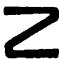
\includegraphics[keepaspectratio]{images/part001_f9c264f7.jpg}}

\begin{enumerate}
\def\labelenumi{(\arabic{enumi})}
\setcounter{enumi}{3}
\tightlist
\item
  Example (3) shows that the \(\mathbf{Z}\) -module \(\mathbf{Q}\) is a flat and faithful module, but not faithfully flat.
\end{enumerate}

PROPOSITION 2. Let E be a faithfully flat right A-module and \(u: \mathbf{N}' \to \mathbf{N}\) a left A-module homomorphism. For \(u\) to be injective (resp. surjective, bijective), it is necessary and sufficient that \(1_{\mathbf{E}} \otimes u: \mathbf{E} \otimes_{\mathbf{A}} \mathbf{N}' \to \mathbf{E} \otimes_{\mathbf{A}} \mathbf{N}\) be so.

This is an immediate consequence of criterion (a) of Proposition 1.

PROPOSITION 3. Let \(0 \to E' \to E \to E'' \to 0\) be an exact sequence of right A-modules. Suppose that \(E'\) and \(E''\) are flat and that one of them is faithfully flat. Then \(E\) is faithfully flat.

We know already that E is flat (§ 2, no. 5, Proposition 5). We verify that E has property (b) of Proposition 1. Let N be a left A-module. As E'' is flat, there is an exact sequence

\[
0 \rightarrow \mathrm{E} ^ {\prime} \otimes_ {\mathrm{A}} \mathrm{N} \rightarrow \mathrm{E} \otimes_ {\mathrm{A}} \mathrm{N} \rightarrow \mathrm{E} ^ {\prime \prime} \otimes_ {\mathrm{A}} \mathrm{N} \rightarrow 0
\]

(§ 2, no. 5, Proposition 4). If \(\mathbf{E} \otimes_{\mathbf{A}} \mathbf{N} = 0\) , it follows that \(\mathbf{E}' \otimes_{\mathbf{A}} \mathbf{N}\) and \(\mathbf{E}'' \otimes_{\mathbf{A}} \mathbf{N}\) are zero; as one of the modules \(\mathbf{E}', \mathbf{E}''\) is faithfully flat, this implies that \(\mathbf{N} = 0\) .

